\documentclass[12pt]{article}

\usepackage[T1]{fontenc}
\usepackage[utf8]{inputenc}
\usepackage[english]{babel}
\usepackage{indentfirst}
\usepackage[margin=2.5cm]{geometry}
\usepackage[hidelinks]{hyperref}
\usepackage{graphicx}
\usepackage{amsmath}

\graphicspath{ {./images/} }

\renewcommand{\baselinestretch}{1.5} % spacing

\usepackage[backend=bibtex, sorting=none]{biblatex}
\bibliography{bibl}

\title{Artificial Intelligence Report - The 15-puzzle}
\author{Aneta Andrzejewska 200285 \and Michał Kącki 203206}
\date{20 November 2018}


\begin{document}

\pagenumbering{gobble}

\maketitle
\newpage

\tableofcontents
\newpage

\pagenumbering{arabic}
\setcounter{page}{3}

\section{Introduction}
\subsection{Background}

The 15-puzzle game is a sliding puzzle consisting of a frame of numbered square tiles in random order with one tile missing \cite{15-puzzle}. The goal of the game is to shift the tiles in such a way that they are in order using the empty space. The game comes in different settings characterised by the number of slides. The two most popular sizes are $3\times3$ and $4\times4$, which are called the 8- and 15-puzzle, respectively.

The n-puzzle game is a popular problem in computer science used to model different algorithms using various heuristics as a means to solve the puzzle. This is possible because all the states, i.e. placings of the slides, which a board for the puzzle can be in, could be represented as nodes of a graph, where every node has three or four children, representing the state of the board after moving the empty space in every direction. Three children are considered when the empty space is located on the border of the board.

\subsection{Goal}

The goal of the laboratory was to implement the 15-puzzle game alongside a few algorithms used for solving it and analyse them in terms of their performance. The considered algorithms were:

\begin{itemize}
    \item Breadth-first search (BFS)
    \item Depth-first search (DFS)
    \item Iterative deepening depth-first search (IDDFS)
    \item Best-first search (BFS)
    \item A*
    \item Simplified Memory Bounded A* (SMA*)
\end{itemize}

In addition to the above requirements, the program should also provide the user with a possibility to choose one of two heuristics for best-first search, A* and SMA*. It should be possible to start the program and pass relevant arguments via the command line. The last requirement was that the program should be able to print the sequence of moves of the empty space leading to obtaining the solved puzzle.

\subsection{Description of the algorithms}

\subsubsection{Breadth-first search (BFS)}

Breadth-first search is the simplest method of traversing a graph. The idea is that each vertex at the present depth needs to be expanded before descending further down the tree. While definitely simple, BFS slows down immensely when the considered graph is too large.

\begin{figure}[h]
    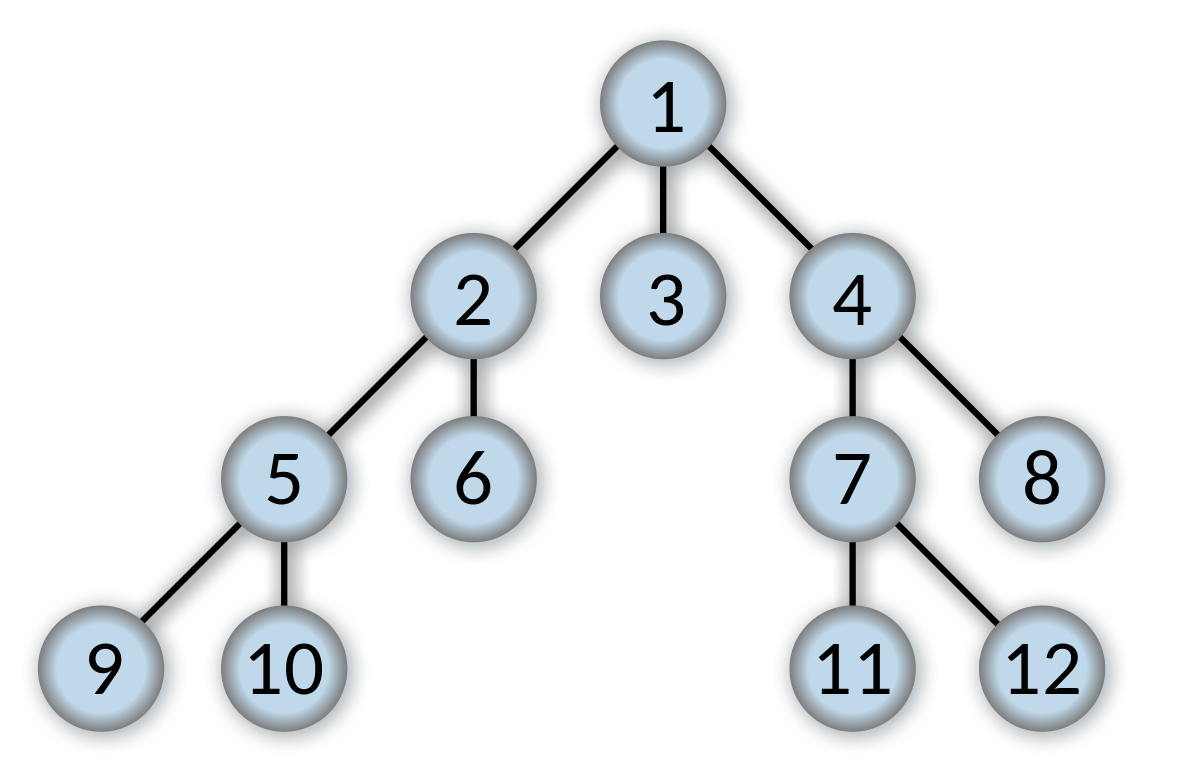
\includegraphics[width=0.75\textwidth]{bfs}
    \centering
    \caption{Breadth-first search traversal order \cite{bfs_image}}
\end{figure}

\subsubsection{Depth-first search (DFS)}

Depth-first search is another simple method of traversing graphs. It differs from the BFS in that it prioritises expanding one path towards the bottom of the graph instead of visiting each vertex at a particular depth first. When a path is completely expanded, the algorithm goes back to expand the omitted nodes.

\begin{figure}[h]
    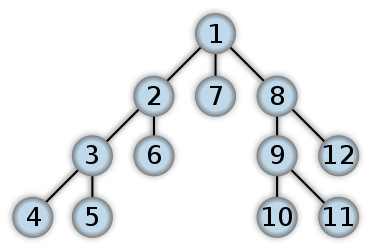
\includegraphics[width=0.75\textwidth]{dfs}
    \centering
    \caption{Depth-first search traversal order \cite{dfs_image}}
\end{figure}

\subsubsection{Iterative deepening depth-first search (IDDFS)}

Iterative deepening depth-first search algorithm is basically the improved version of DFS in that it also utilises the strategy present in BFS. IDDFS uses a parameter called ``depth limit'', which tells the algorithm how deep to traverse down the tree before running BFS on a particular level. IDDFS may be thought of as a combination of DFS and BFS - it takes space-efficiency from the former and completeness from the latter effectively performing a lot better than the aforementioned algorithms.

\begin{figure}[h]
    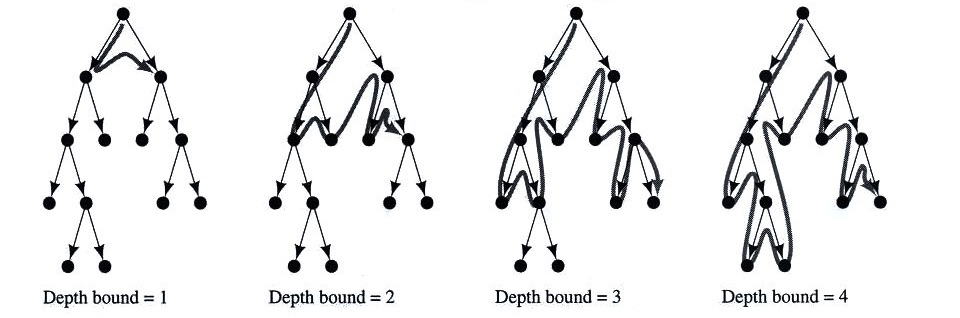
\includegraphics[width=0.75\textwidth]{iddfs}
    \centering
    \caption{Iterative deepening depth-first search traversal order \cite{iddfs_image}}
\end{figure}

\subsubsection{Best-first search (BFS)}

Best-first search is quite different from all the above methods. To arrive at a solution it uses a heuristic evaluation function telling the algorithm which vertex should now be expanded. There exists a plethora of different heuristics to choose from. One of the most popular is called a ``pure heuristic''. When utilising that heuristic, the algorithm tries to assess how close a particular path is to a solution and first chooses those that are the closest. When using heuristics, each vertex has a weight associated with it.

\begin{figure}[h]
    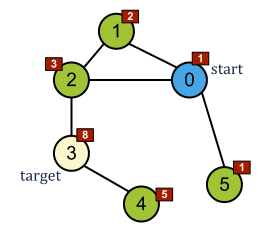
\includegraphics[scale=0.75]{bfs2}
    \centering
    \caption{Best-first search traversal order showing the weights of the nodes \cite{bfs2_image}}
\end{figure}

\subsubsection{A*}

A* algorithm is a kind of best-first search as it uses heuristics as well. However, instead of considering only a path from the current node to a solution, the whole cost of arriving at the currently considered vertex is also taken into consideration. A* strategy is described by the following equation:

\[
f(n) = g(n) + h(n),
\]
where $n$ indicates the next vertex on the path, $g(n)$ is the cost from the root vertex to $n$ and $h(n)$ is the aforementioned heuristic function evaluating the cost of the cheapest path from the vertex $n$ to the solution.

\begin{figure}[h]
    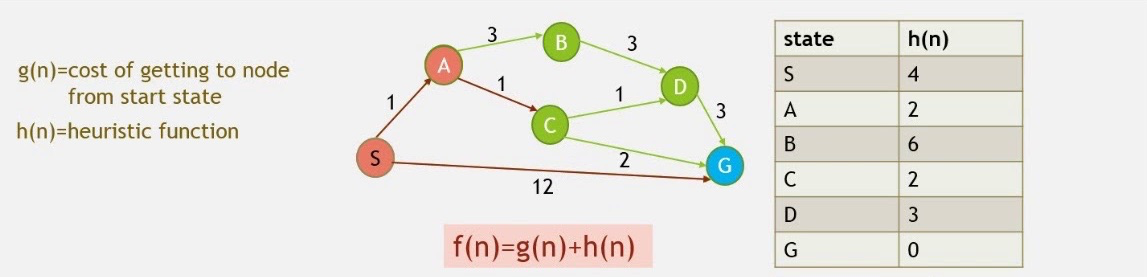
\includegraphics[width=\textwidth]{astar}
    \centering
    \caption{A* traversal order \cite{astar_image}}
\end{figure}

\subsubsection{Simplified Memory Bounded A* (SMA*)}

Simplified Memory Bounded A* is the successor of MA* which takes the concept of A* and applies memory bounds on the container storing vertices yet to be visited. When the container is full, the most costly nodes (those with the highest f-cost) are dropped to make a place for the nodes that might be a better choice. To prevent infinite looping the f-cost values are backed up through the tree. When it is needed, some nodes are re-expanded. SMA* simplifies the logic of MA* and in fact, performs better than its overcomplicated predecessor. First of all, it uses a binary tree to store the list of vertices that need to be expanded, which is a more efficient data structure than the one originally used in MA*. Also, the backup procedure is started only when a vertex has been fully expanded, which speeds up the execution time of the algorithm \cite{GCAI2017:Enhanced_Simplified_Memory_bounded_Star}.

\begin{figure}[h]
    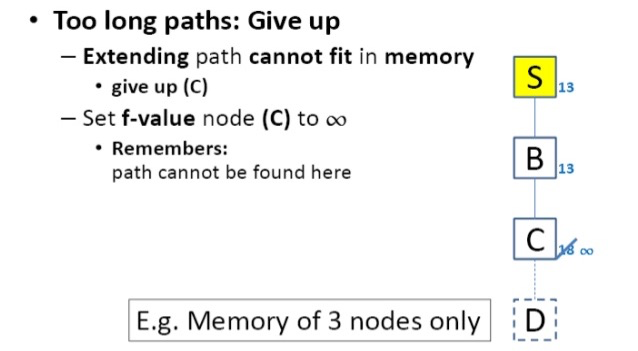
\includegraphics[width=0.75\textwidth]{smastar}
    \centering
    \caption{SMA* logic \cite{smastar_image}}
\end{figure}

\section{Implementation}

\subsection{Language}

The program has been written in Eclipse IDE using Java programming language with JDK 8.

\subsection{Functional requirements}
\subsubsection{Command line arguments}

The program can be started from the command line and takes the following parameters:

\begin{itemize}
    \item -b / --bfs order (BFS)
    \item -d / --dfs order (DFS)
    \item -i / --idfs order (IDDFS)
    \item -h / --bf id-of-heuristics (best-first search)
    \item -a / --astar id-of-heuristics (A*)
    \item -s / --sma id-of-heuristics (SMA*)
    \item --help (printing help)
\end{itemize}

BFS, DFS and IDDFS require the order in which successors of given state are processed to be passed. ``R'' indicates that the nodes can be chosen randomly, whereas a string ``R L U D'' means the following search order: right, left, up, down.

Best-first search, A* and SMA* require an ID of a heuristic to be passed. The implemented ones are:

\begin{itemize}
    \item 0 / --zero (zero heuristics)
    \item  1 / --inpos (incorrect position heuristics)
    \item 2 / --mand (Manhattan distance heuristics)
\end{itemize}

Zero heuristics means that every node answers with a value of 0, which means that every node is considered as good as the others.

Incorrect position heuristics calculates how many tiles are in the wrong position - the less the value of the function, the better the tile is.

Manhattan distance heuristics answers with the sum of distances from each tile's position to its correct place applying the Manhattan distance formula:

\[
    d(p, q) = |p_1 - q_1| + |p_2 - q_2|,
\]

where $d$ is the distance, $p$ and $q$ are the considered vectors and $(p_1, p_2)$, $(q_1, q_2)$ are their components.

In the first line of standard input two integer values, R C are given: row count and column count, respectively, defining frame size. Subsequent R lines of standard input contain C space separated integer values describing a piece in the puzzle. Value 0 denotes the empty space in the given frame.

Additionally, the second small program has been created, namely a ``viewer''. The viewer allows users to see what moves were performed to arrive at a solved board.

\subsection{Output}

When the first program finishes its work, it displays four lines of text. In the first line, a size of the puzzle is shown (rows $\times$ columns). The second line contains the initial order of tiles in the board. The third line contains the length of the sequence of moves leading to a correct solution, whereas the fourth line is filled with the aforementioned sequence of moves.

The same information is also saved to a file which can be used by the viewer, where each consecutive permutation, i.e. the state of the board, is displayed every second.

\newpage
\listoffigures
\newpage
\printbibliography

\end{document}




